
\chapter{Sistemi anti-DDoS: stato dell'arte}
% attacchi e contromisure sui ddos

% Quando Internet è stato inventato non si pensava a questo problema e non sono state implementate difese

\section{Riconoscimento DDoS}

% \cite{ddos_motivations} pagina 16, \cite{ddos_survey_4} pagina 66
La fase di riconoscimento degli attacchi DDoS è un importante passo per permettere la successiva mitigazione, questa fase diventa più facile maggiormente ci avviciniamo alla vittima dell'attacco, ma viceversa più ci si allontana dalla sorgente dell'attacco e più diventa difficile identificarla. In letteratura esistono due tecniche per identificare i flussi malevoli: signature-based detection e anomaly-based detection.

\subsection{Signature-based detection}

La signature-based detection è un meccanismo che si basa sul riconoscimento di attacchi DDoS conosciuti, differenziando la loro firma dai normali flussi della rete. Queste soluzioni hanno un buon successo con attacchi DDoS noti, ma non sono in grado di rilevare nuove tipologie di attacco delle quali non si conosce ancora la signature. Questi sistemi si possono basare su pattern matching (es. Bro/Zeek), su regole (es. Snort, Suricata), sulla correlazione di informazioni di management sul traffico o sull'analisi spettrale.
% todo: rivedere le ultime due perché non so bene cosa siano

\subsection{Anomaly-based detection}

I sistemi basati sul rilevamento delle anomalie possono riconoscere anche attacchi non conosciuti, basandosi su delle soglie per differenziare il traffico normale da quello malevolo, ma la scelta dei limiti oltre i quali considerare il traffico anomalo è una grande sfida per questa tipologia di tecniche.
I metodi più diffusi si basano su metodi statistici, di data mining o intelligenze artificiali.

\section{Contromisure attacchi DDoS}

Gli attacchi DDoS si raggruppano ad imbuto dalle sorgenti verso la vittima, per questa ragione più si è vicini alla vittima e più l'attacco sarà facile da riconoscere, ma più difficile da mitigare. Per questa ragione le tecniche di mitigazione vengono suddivise in base al luogo in cui vengono azionate.

\begin{figure}[]
    % todo: capire come gestire citazioni imsmagini a livello di copyright
    \label{fig:classificazione_ddos}
    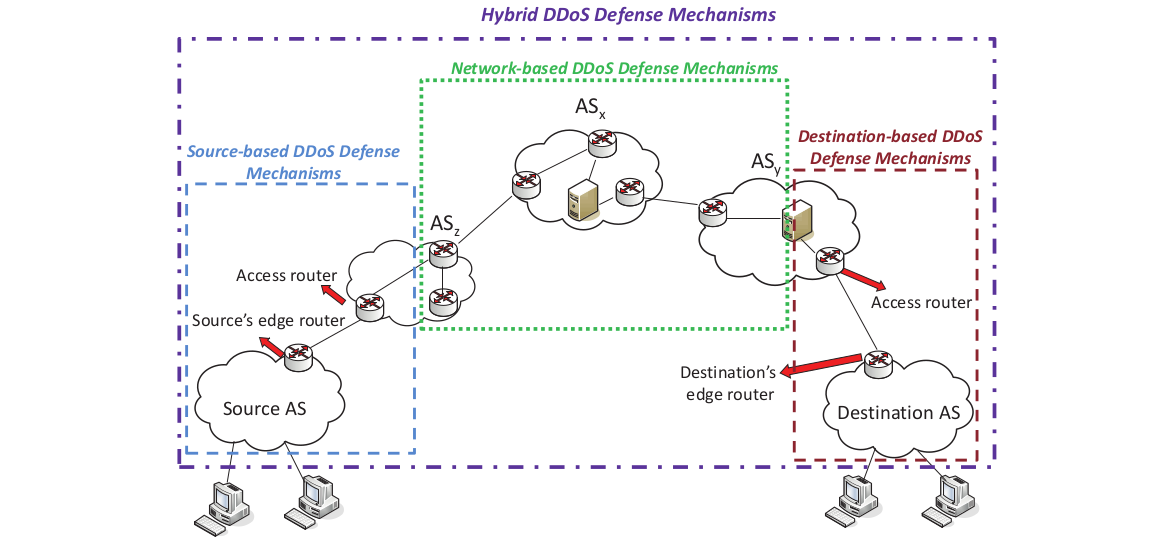
\includegraphics[width=\hsize]{images/ddos/classificazione_difese.png}
    \caption{Classificazione dei sistemi di difesa in base al luogo di applicazione \cite{ddos_survey_1}}
    \centering
\end{figure}

\subsection{Soluzioni alla sorgente}
Questa tipologia di soluzioni sono adottate vicino alle sorgenti dell'attacco per impedire agli utenti di una sottorete di generare attacchi DDoS. Queste soluzioni possono essere applicate agli edge router degli Autonomous System (AS) di accesso.

Degli esempi di soluzioni sono \cite{ddos_survey_1}:

% todo: completare elenco delle soluzioni alla sorgente
\begin{itemize}
    \item Filtri in ingresso e uscita agli edge router delle sorgenti: gli attacchi che si basano sulla riflessione sfruttano la tecnica dell'ip spoofing, lo scopo di questi filtri è di bloccare il traffico che lo utilizza senza interferire sul traffico legittimo.
    \item D-WARD: sistema che mira a rilevare attacchi di tipo DDoS flooding monitorando il traffico in ingresso e uscita e comparandolo con dei flussi normali di traffico. I flussi sono filtrati se non rispettano il modello. Per esempio può essere imposto un rapporto massimo tra pacchetti inviati e ricevuti per un flusso TCP che se superato può segnalare il flusso come anomalo.
    \item MULTOPS (MUlti-Level Tree for Online Packets Statistics): è un'euristica e un struttura dati che permette di rilevare attacchi provenienti da una subnet. Normalmente il traffico in una direzione è proporzionale a quello in quella opposta, una significativa differenza possono indicare che la rete è la sorgente o la vittima di un attacco DDoS.
    \item MANAnet’s Reverse Firewall: è un firewall che a differenza di quelli tradizionali, protegge l'esterno dal traffico in uscita dalla subnet.
\end{itemize}

I problemi di questa soluzione sono che per permettere una copertura totale, questi meccanismi dovrebbe essere implementatati su tutti gli edge router di tutti gli AS di accesso, inoltre è difficile differenziare il traffico legittimo, da quello malevolo e non meno importante non è chiaro chi sia il responsabile del mantenimento economico di questo servizio \cite{ddos_survey_1}.

\subsection{Soluzioni alla destinazione}

Esistono soluzioni che si possono applicare agli edge router della vittima, possono analizzare il suo comportamento, il suo traffico usuale e riconoscere le anomalie \cite{ddos_survey_1,ddos_survey_2}.
Delle soluzioni posizionate in questi luoghi possono essere dei proxy, firewall che gestiscono le connessioni semi aperte in caso di syn flood oppure l'utilizzo sistemi di tracciamento implementati in alcuni router (in caso di ip spoofing), per risalire alla vera sorgente dell'attacco e bloccarla. % todo: non so come concludere le soluzioni alla destinazione, sicuramente c'è qualche meccanismo che ho dimenticato \cite{ddos_survey_2, ddos_survey_1}

% todo: potrei descriverli in maniera più dettagliata 

Questi sistemi di difesa possono diventare i target degli attacchi, poiché spesso richiedono una grande quantità di memoria e potenza di processamento per effettuare le osservazioni delle misure statistiche \cite{ddos_survey_4}.

\subsection{Soluzioni sulla rete}

I sistemi anti-DDoS sulla rete si basano sui router o su firewall installati sulla rete dell'operatore.
Una prima soluzione adottata è quella del Router based packet filter, la quale si basa sui criteri dell'ingress filtering, ma applicandola ai router nel core della rete. Il traffico per ogni link tendenzialmente viene generato da un ristretto intervalli di indirizzi ip, quando appare un indirizzo ip sospetto viene filtrato, questa soluzione è adatta a rilevare attacchi che utilizzano ip spoofing, ma è inutile nel caso di utilizzo di ip genuini.
Altre soluzioni mirano ad identificare i router nel core di internet che sono stati compromessi e si comportano in modo anomalo, oppure mirano all'installazione di detection systems (DSs) i quali permettono di rilevare pattern anomali, ma sono computazionalmente molto dispendiosi.

I problemi di questa soluzione è l'introduzione di un overhead per il processamento sui router, inoltre il rilevamento degli attacchi è difficile a causa dei dati troppo poco aggregati.

\subsection{Soluzioni distribuite}

Le soluzioni distribuite creano una cooperazione tra i luoghi di installazione delle difese. Alla sorgente vengono installati i sistemi di difesa per filtrare l'attacco, mentre sulla rete della vittima viene effettuato il riconoscimento dell'attacco. Questa soluzione porta sia il vantaggio della facilità di riconoscimento degli attacchi possibile alla destinazione, sia l'efficienza dei sistemi per mitigare gli attacchi alla sorgente.
Gli svantaggi di questa soluzione sono la complessità e l'overhead dovuto alla comunicazione tra le componenti distribuite e il bisogno di comunicazioni/componenti fidati tra le varie parti responsabili della cooperazione.
Degli esempi di soluzioni distribuite sono i seguenti:
\begin{itemize}
    \item Hybrid packet marking and throttling/filtering mechanisms: sono meccanismi in cui viene rilevato l'attacco vicino alla vittima, la quale informa i router in upstream di limitare o filtrare quel traffico. Degli esempi di applicazione di questa tecnica sono:
    \begin{itemize}
        \item Aggregate-based  congestion Control (ACC and Pushback: rileva un sottogruppo di traffico aggregato secondo alcune caratteristiche e richiede ai router in upstream di limitare o filtrare quel traffico.
        \item Attack diagnosis (AD) and parallel-AD: la vittima attiva l'AD quando un attacco viene rilevato, mandando i comandi correlati ai router in upstream, che contrassegneranno i pacchetti in transito con l'interfaccia di provenienza. Completato il traceback fino alla sorgente verrà mandato il comando AD per filtrare i pacchetti in arrivo alla sorgente.
        % todo: track
        \item TRACK
    \end{itemize}
    \item DEFensive Cooperative Overlay Mesh (DEFCOM): è un framework distribuito per abilitare lo scambio di informazioni tra tutti i nodi di difesa. Questo sistema prova a passare da un'architettura di difesa isolata ad una distribuita.
    \item Capability-based mechanisms: questo meccanismo permette alla destinazione di autorizzare esplicitamente il traffico che vuole ricevere.
    \item StopIt: meccanismo distribuito che prevede un sistema di autenticazione: tramite il quale viene prevenuto l'ip spoofing, e a dei pacchetti costruiti per essere inoltrati ai router in upstream che permettono il filtraggio del traffico il più vicino possibile alla sorgente del traffico.

\end{itemize}

\section{Momenti in cui mettere in atto le difese}

Esistono più momenti in cui è opportuno mettere in atto le difese contro attacchi DDoS e un buon sistema deve agire su tutti.
Il primo momento è prima dell'attacco (attack prevention), in cui vengono installati sistemi di monitoring, sistemi da usare in caso di emergenza, meccanismi per tollerare l'attacco (firewall, IDS, filtri, load balancer e flow control, strategie per identificare gli utenti legittimi e protezioni lato server). Successivamente durante l'attacco devono essere lanciate le adeguate contromisure e dopo l'attacco il sistema di difesa deve identificare la fonte e provvedere con le opportune contromisure, anche collaborando con altri segnalare l'attacco per permettere di difendersi da successivi.

\begin{figure}[]
    \label{fig:albero_difese}
    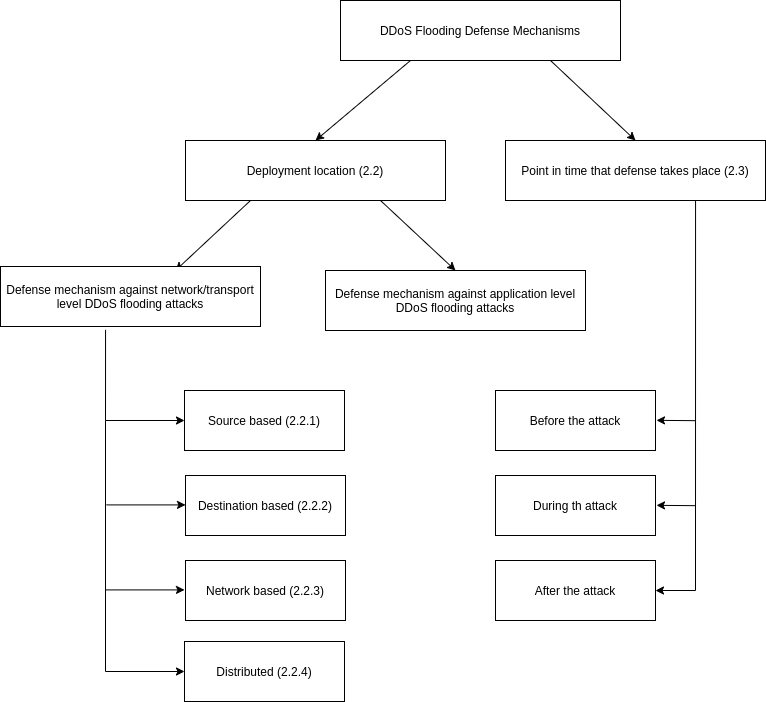
\includegraphics[width=\hsize]{images/ddos/ddos_flooding_defence.png}
    \caption{Meccanismi di difesa contro DDoS di tipo flooding.}
    \centering
\end{figure}

% \section{Tolleranza}
